\documentclass[9pt]{pnas-new}
% Use the lineno option to display guide line numbers if required.
% Note that the use of elements such as single-column equations
% may affect the guide line number alignment. 

\RequirePackage[english,slovene]{babel} % when writing in slovene
%\RequirePackage[slovene,english]{babel} % when writing in english

\templatetype{pnasresearcharticle} % Choose template 
% {pnasresearcharticle} = Template for a two-column research article
% {pnasmathematics} = Template for a one-column mathematics article
% {pnasinvited} = Template for a PNAS invited submission

\selectlanguage{slovene}
\etal{in sod.} % comment out when writing in english
\renewcommand{\Authands}{ in } % comment out when writing in english
\renewcommand{\Authand}{ in } % comment out when writing in english

\newcommand{\set}[1]{\ensuremath{\mathbf{#1}}}
\renewcommand{\vec}[1]{\ensuremath{\mathbf{#1}}}
\newcommand{\uvec}[1]{\ensuremath{\hat{\vec{#1}}}}
\newcommand{\const}[1]{{\ensuremath{\kappa_\mathrm{#1}}}} 

\newcommand{\num}[1]{#1}

\graphicspath{{./fig/}}

\title{Modeliranje evakuacije ljudi pred napadalcem z uporabo mehke logike}

% Use letters for affiliations, numbers to show equal authorship (if applicable) and to indicate the corresponding author
\author{Martin Božič}
\author{Marija Marolt}
\author{Jakob Maležič}

\affil{Poročilo seminarske naloge pri predmetu Skupinsko vedenje} 

% Please give the surname of the lead author for the running footer
\leadauthor{Novak} 

\selectlanguage{english}

% Please add here a significance statement to explain the relevance of your work
\significancestatement{Crowd evacuation with Assailants via a Fuzzy logic approach}{TODO: Add english abstract?}{Collective behaviour | Crowd evacuation | Fuzzy logic}

\selectlanguage{slovene}

% Please include corresponding author, author contribution and author declaration information
%\authorcontributions{Please provide details of author contributions here.}
%\authordeclaration{Please declare any conflict of interest here.}
%\equalauthors{\textsuperscript{1}A.O.(Author One) and A.T. (Author Two) contributed equally to this work (remove if not applicable).}
%\correspondingauthor{\textsuperscript{2}To whom correspondence should be addressed. E-mail: author.two\@email.com}

% Keywords are not mandatory, but authors are strongly encouraged to provide them. If provided, please include two to five keywords, separated by the pipe symbol, e.g:
\keywords{Skupinsko vedenje | Evakuacija ljudi | Mehka logika } 

\begin{abstract}
%To sem na hitro nekaj nakracal
Vsako leto se po celem svetu zgodi veliko napadov, kjer je ustreljenih in poškodovanih veliko ljudi. V tem članku, s pomočjo mehke logike, zgradimo različne modele, s katerimi lahko simuliramo takšne napade. Najprej predstavimo manjše modele, ki želijo doseči specifičen cilj - izogibanje oviram, iskanje poti in doseganje točke v prostoru. Te modele nato združimo v celoto tako, da jih ustrezno utežimo. Model testiramo in simuliramo v različnih prostorih z različnimi parametri. Za boljše razumevanje simulacije pripravimo tudi uporabniški vmesnik, ki simuliran napad vizualno prikaže. Naš model primerjamo še z ostalimi obstoječimi modeli.
\end{abstract}

\dates{\textbf{\today}}
\program{BM-RI}
\vol{2020/21}
\no{CB:GB} % group ID
%\fraca{FRIteza/201516.130}

\begin{document}

% Optional adjustment to line up main text (after abstract) of first page with line numbers, when using both lineno and twocolumn options.
% You should only change this length when you've finalised the article contents.
\verticaladjustment{-2pt}

\maketitle
\thispagestyle{firststyle}
\ifthenelse{\boolean{shortarticle}}{\ifthenelse{\boolean{singlecolumn}}{\abscontentformatted}{\abscontent}}{}

% If your first paragraph (i.e. with the \dropcap) contains a list environment (quote, quotation, theorem, definition, enumerate, itemize...), the line after the list may have some extra indentation. If this is the case, add \parshape=0 to the end of the list environment.
\dropcap{Z}biranje velikih gruč ljudi na javnih mestih je postalo nekaj neizogibnega. Na avtobusnih postajah, na železniški postaji, v velikih trgovskih centrih ali pa na koncertih in tekmah. Slednje lahko predstavlja veliko nevarnost za ljudi, kot tudi velik izziv za organizatorje in nadzornike takšnih javnih prostorov. Posebno pozornost je vredno nameniti predvidevanju potencialnih kriznih situacij, pri katerih je treba upoštevati nerazumno vedenje množice, ki nastopi kot posledica tesnobe in panike. V tem obziru je ključnega pomena razumevanje in razlikovanje značilnosti vedenja ljudi v običajnih ter kriznih situacijah.

Pri analizi dosedanjih napadov na množice, kot so streljanje v šolah~\cite{shootingWiki} in teroristični napadi na železniške postaje~\cite{CunmingWiki}, je prišlo do nekaj pomembnih spoznanj. Iracionalno evakuacijsko vedenje, slaba presoja varnosti stanovalcev ter malomarnost in nerazumne arhitekturne odločitve so vidno povečali škodo povzročenih napadov.

Preučevanje evakuacije množice vključuje lahko temelji na realnih poskusih ali računalniški simulaciji. Izvedeni so bili poskusi evakuacije pri zastoju na hodniku~\cite{bottlenecks2005}, v učilnici~\cite{classroom2008} ter nebotičniku~\cite{building2012}, ki so razkrili nekaj tipičnih vedenjskih vzorcev pri evakuaciji, kot so na primer tvorjenje vrst po principu zadrge~\cite{bottlenecks2005}, prilaščanje izhoda in čas priprave na evakuacijo~\cite{classroom2008}. V zadnjih nekaj desetletjih se vse bolj uporablja različne simulacijske modele. Helbing~\cite{Helbing2000} je predstavil model, ki simulira obnašanje ljudi v paniki pri evakuaciji. Pojasnil je zakaj pride do zastojev in poiskal optimalno rešitev. Varas~\cite{Varas2007} je uporabil model za odločanje s celičnim avtomatom za evakuacije sobe z ovirami. Upošteval je nerazumno vedenje v primeru panike in ob srečanju z oviro dodal faktor naključnosti reakcije v naslednjem koraku. Liu~\cite{Liu2009} je kasneje model nekoliko prilagodil. Obravnaval je tudi gostoto ljudi okoli izhoda. Poleg omenjenih so bili za preučevanje tega področja uporabljeni tudi drugi modeli. Izkazalo se je, da so rezultati močno odvisni od situacije in okolja.



\section*{Metode}
Za simulacijo gruč ljudi smo morali najprej pripraviti model za vodenje posameznega človeka kot tudi napadalca.

V študijah so pokazali, da je vid glavni vir informacij, na podlagi katerih, se človek v kriznih situacijah odloča o svojih dejanjih \cite{brcdp2018, mht2011}. Zato smo tudi mi, zgradili modele, ki se odločajo na podlagi okolice, ki jo človek lahko vidi.

V osnovi ljudi razdelimo v tri kategorije. V tretjo kategorijo uvrščamo vse ljudi, kateri se v trenutni situaciji še ne zavedajo prisotnosti napadalca. Takoj, ko se ti ljudje zavedajo napadalca, v svojem vidnem polju ga pa še ne vidijo, preidejo v drugo kategorijo. V prvo kategorijo pa uvrščamo vse ljudi, ki napadalca vidijo, ali pa so ga videli v bližnji preteklosti in so s tem v napadalčevi neposredni nevarnosti. Ko človek enkrat preide v prvo ali drugo kategorijo, v trenutni simulaciji več ne more preiti v tretjo kategorijo ljudi.

\begin{figure}
	\centering
	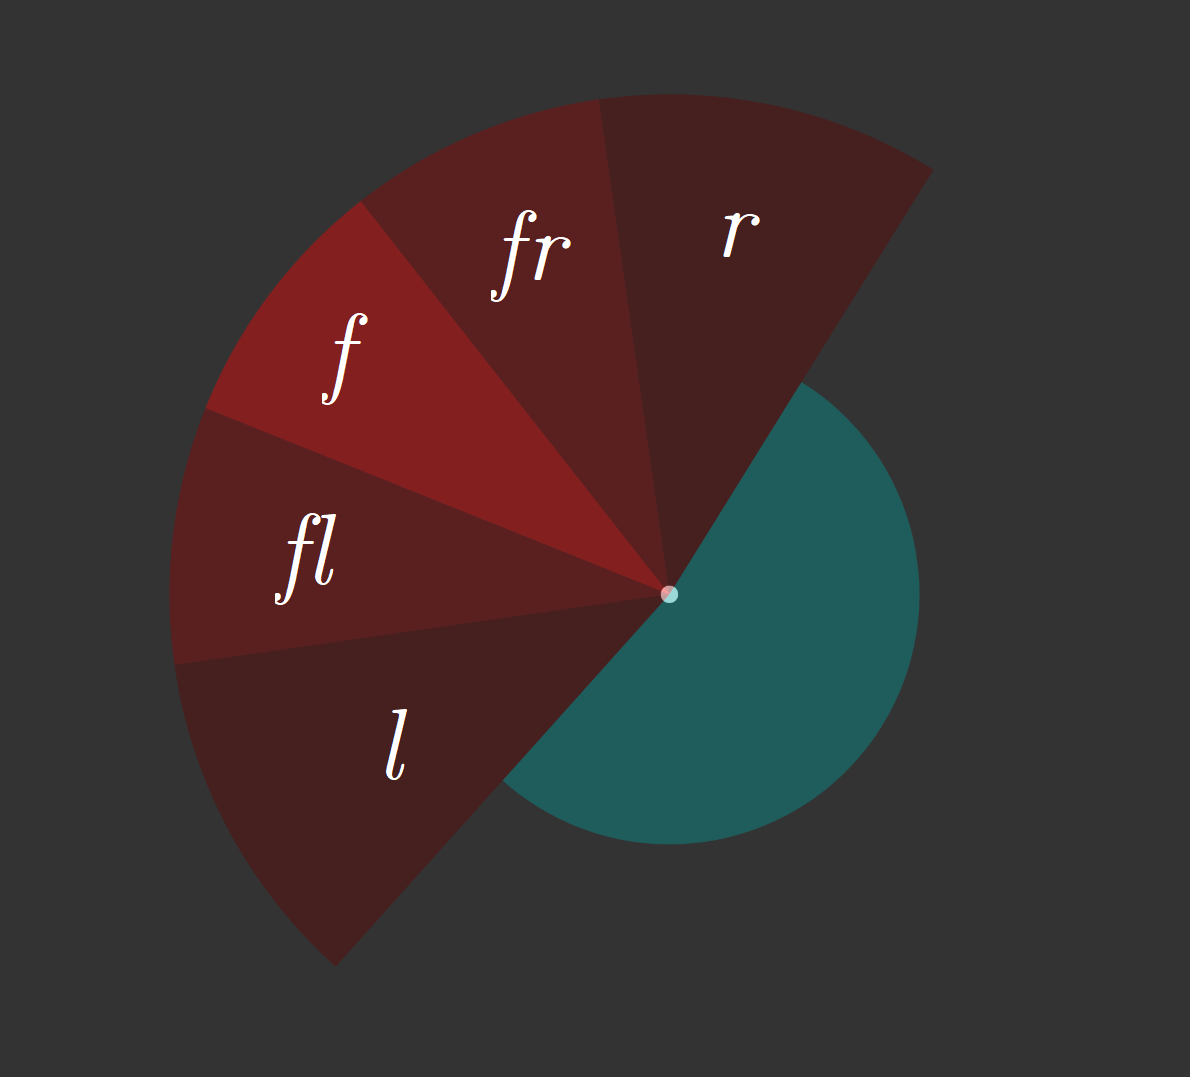
\includegraphics[scale=0.3]{fig/vision_field.PNG}
	\caption{Vidno polje osebe, ki je razdeljeno na sektorje.}
	\label{fig:vision_field}
\end{figure}

\subsection*{Mehka logika}
\label{mehka_logika}
Informacija, ki jo ljudje pridobimo iz okolice je odvisna od našega zaznavanja sveta in v večini primerih ni odvisna od meritev. Kako pridobljena informacija vpliva na posameznika pa je težko določiti s količino, saj se zmožnost zaznavanja razlikuje med posamezniki. Zato je smiselno, da takšne \textbf{POJAVE} opišemo z besedami in ne izmerljivimi količinami. Slednje lažje opišemo z množico mehkih logik, ki jo je predstavil Zadeh \cite{ZADEH1965338} in se uporablja na različnih področjih. Največ se uporablja v odločilnih sistemih \cite{Dong2013}, pri ocenjevanju zmogljivosti \cite{HWWDGHJZN1969}, napovedovalnih kontrolnih sistemih \cite{en10060794} ipd. Metoda množice mehkih logik je tudi veliko bolj robustna pri uporabi netočnih in negotovih informacij, ki se jim pri sistemih, ki so odvisni od zaznavanja okolice, ne moremo izogniti.

\subsection*{Lokalno izogibanje oviram}
\label{lokalno_izogibanje_oviram}
Metoda lokalnega izogibanje oviram poskrbi, da se osebe izognejo oviram, ki se nahajajo pred njimi in so dovolj blizu, da jih oseba zazna. Metoda deluje na podlagi vnaprej določenih pravil mehke logike. Vhode predstavljajo najbližje ovire v posameznih sektorjih vidnega polja, izhoda pa sta smer ($\alpha$) in hitrost gibanja ($V$). Vhodi so predstavljeni z mehko množico \{BLIZU, DALEČ\}, izhoda pa sta predstavljena z mehkima množicama \{Močno-Poz, Malo-Poz, Nič, Malo-Neg, Močno-Neg\} in \{USTAVITEV, POČASI, HITRO\}. Pravila mehke logike metode lokalnega izogibanja oviram lahko sedaj povzamemo z:
\begin{equation}
\label{lokalno_izogibanje_oviram_summarize}
\begin{bmatrix}
\delta_{\alpha}\\
\delta_{V}
\end{bmatrix} = R_{0} (d_{o}^l, d_{o}^fl, d_{o}^f, d_{o}^fr, d_{o}^r)
\end{equation}

Z opisanimi mehkimi množicami dobimo 32 (oziroma $2^5$) pravil ($R_0$), ki so opisana v tabeli \ref{rules_obstacle_avoidance_behaviour}.

\begin{table}[]
\centering
\begin{tabular}{|l|lllll|ll|}
\hline
\textbf{Zap. št.} & \multicolumn{5}{l|}{\textbf{Vhod}} & \multicolumn{2}{l|}{\textbf{Izhod}} \\ 
\cline{2-8} 
\textbf{pravila} & ${d_l}$ & ${d_{fl}}$ & ${d_{fl}}$ & ${d_{fl}}$ & ${d_{fl}}$ & ${\alpha}$ & V \\ 
\hline
1   & BLIZU & BLIZU & BLIZU & BLIZU & BLIZU & Nič           & USTAVITEV  \\ \hline
2   & BLIZU & BLIZU & BLIZU & BLIZU & DALEČ & Močno-Poz     & POČASI     \\ \hline
3   & BLIZU & BLIZU & BLIZU & DALEČ & BLIZU & Malo-Poz      & POČASI     \\ \hline
4   & BLIZU & BLIZU & BLIZU & DALEČ & BLIZU & Močno-Poz     & POČASI     \\ \hline
5   & BLIZU & BLIZU & BLIZU & DALEČ & BLIZU & Nič           & HITRO      \\ \hline
\dots & \dots  & \dots  & \dots  & \dots  & \dots  & \dots  & \dots      \\ \hline
31  & DALEČ & DALEČ & DALEČ & DALEČ & BLIZU & Nič           & HITRO      \\ \hline
32  & DALEČ & DALEČ & DALEČ & DALEČ & DALEČ & Nič           & HITRO      \\ \hline
\end{tabular}
\caption{Tabela predstavlja sistem pravil mehke logike pri metodi lokalnega izogibanja oviram.}
\label{rules_obstacle_avoidance_behaviour}
\end{table}

\subsection*{Iskanje poti}
\label{iskanje_poti}
Pri metodi iskanja poti na spremembo trenutne hitrosti in smeri posamezne osebe najbolj vplivajo hitrosti in smeri ostalih oseb v vidnem spektru osebe. Tako bi pri metodi iskanja poti na trenutno osebo najbolj vplivala oseba, ki se proti izbrani osebi premika z veliko hitrostjo v nasprotni smeri. Metoda vedno vodi posameznika po najvarnejši poti, tako da se vedno izogiba področjem z visoko negativno energijo. Moč negativne energije se izračunava sproti in je odvisna od trenutnega vpliva ovir in trenutne nevarnosti trčenja posameznika z ostalimi osebami. Kot vpliv ovire v večini upoštevamo zidove, pohištvo in ostale stacionarne reči v vidnem sektorju posameznika. Vpliv ovir označimo z oznako ${(OI^*)}$, pri čemer sistem mehke logike za izračun trenutnega vpliva ovir opišemo z enačbo \ref{OI_equation}.

\begin{equation}
\label{OI_equation}
OI_{i}^* = R_{1}(\phi^*_{oi}, d^*_{oi})
\end{equation}

${\phi^*_{oi}}$ predstavlja v katerem kotu vidnega spektra posameznika se ovira nahaja, ${d^*_{oi}}$ predstavlja razdaljo od posameznika do posamezne ovire in ${R_{1}}$ predstavlja zbirko pravil mehke logike.


Nevarnost trčenja opazovane osebe z drugo osebo v prostoru označimo z oznako ${(CR^*)}$, pri čemer sistem mehke logike opišemo z enačbo \ref{CR_equation}.

\begin{equation}
\label{CR_equation}
CR_{j}^* = R_{2}(d^*_{oi}, V_{j}^*, \theta_{pj}^*)
\end{equation}

${V_{j}^*}$ predstavlja trenutno hitrost j-te osebe, ${\theta_{pj}^*}$ predstavlja kot med smerjo gibanja j-te osebe glede na trenutno opazovano osebo in ${d^*_{pj}}$ predstavlja razdaljo od j-te osebe do trenutno opazovane osebe. ${R_{2}}$ predstavlja zbirko pravil mehke logike. Celotno negativno energijo trenutne opazovane osebe izračunamo z enačbo \ref{NE_equation},

\begin{equation}
\label{NE_equation}
NE^* = k_{w} \cdot OI^* + (1 - k_{w}) \cdot CR^*
\end{equation}

, kjer ${OI^*}$ predstavlja vsoto vseh ${OI_{i}^*}$, za vsak predmet i v vidnem spektru osebe in ${CR^*}$ predstavlja vsoto vseh izračunanih nevarnosti trčenja ${CR_{j}^*}$, za vsako j-to osebo, ki se giblje v vidnem prostoru trenutne osebe. ${k_{w}}$ predstavlja faktor uteži, s katerim lahko nadziramo pomembnost vrednosti OI in CR.


\subsection*{Doseganja cilja}
\label{doseganje_cilja}
Pri metodi doseganja cilja, se opazovana oseba vedno nagiba k temu, da se pomika proti končnemu cilju. Opišemo jo z ${d_g}$, ki predstavlja razdaljo do cilja g in ${\gamma_{g}}$, ki predstavlja kot, glede na orientacijo trenutne osebe in smerjo cilja. Razdaljo ${d_g}$ opišemo z dvema \{BLIZU, DALEČ\}, kot ${\gamma_{g}}$ pa s petimi \{Močno-Neg, Malo-Neg, Nič, Malo-Poz, Močno-Poz\} stanji mehke logike. Sistem pravil mehke logike pri metodi doseganja cilja je predstavljen v tabeli \ref{rules_goal_seeking_behaviour}. Pri čemer ${\alpha}$ predstavlja končni kot in V predstavlja hitrost premika opazovane osebe.

% \usepackage{multirow}
\begin{table}[]
\centering
\begin{tabular}{|l|ll|ll|}
\hline
\textbf{Zap. št.} & \multicolumn{2}{l|}{\textbf{Vhod}} & \multicolumn{2}{l|}{\textbf{Izhod}} \\ \cline{2-5} 
\textbf{pravila} & ${\gamma_{g}}$          & ${d_g}$          & ${\alpha}$           & V          \\ \hline
1                            & Močno-Poz  & BLIZU & Močno-Neg  & USTAVITEV  \\ \hline
2                            & Močno-Poz & DALEČ & Močno-Neg   &  POČASI           \\ \hline
3                            & Malo-Poz &  BLIZU &   Malo-Neg   &  POČASI   \\ \hline
4                            & Malo-Poz & DALEČ &  Malo-Neg  &  POČASI   \\ \hline
5                            & Nič      &  BLIZU &  Nič    &   HITRO    \\ \hline
6                            & Nič      & DALEČ  &  Nič    &   HITRO  \\ \hline
7                            & Malo-Neg & BLIZU & Malo-Poz    &  POČASI   \\ \hline
8                            & Malo-Neg & DALEČ & Malo-Poz   &  POČASI    \\ \hline
9                            & Močno-Neg & BLIZU &  Močno-Poz   & USTAVITEV \\ \hline
10                           & Močno-Neg & DALEČ  &  Močno-Poz   &  POČASI   \\ \hline
\end{tabular}
\caption{Tabela predstavlja sistem pravil mehke logike pri metodi doseganja cilja.}
\label{rules_goal_seeking_behaviour}
\end{table}

\subsection*{Utežena vsota}
Končno hitrost V in končni kot premika ${\alpha}$ trenutne osebe izračunamo z metodo utežene vsote rezultatov metode umikanja oviram \ref{umikanje_oviram}, metode iskanja poti \ref{iskanje_poti} in metode doseganja cilja \ref{doseganje_cilja}. Pomembnost rezultata vsake metode utežimo s faktorji ${\delta_{ao}}$, ${\delta_{ap}}$ in ${\delta_{ag}}$, ki sproti utežujejo pomembnost vsake posamezne metode mehke logike. Vsak faktor opišemo s tremi stanji mehke logike, \{MANJŠI, SREDNJI, VELIK\}. Vrednosti faktorjev določamo sproti po enačbi \ref{delta_equation},

\begin{equation}
\label{delta_equation}
\begin{bmatrix}
\delta_{ao}\\
\delta_{ap}\\
\delta_{ag}
\end{bmatrix} = R_{5} (d_{o}^f, \overline{NE^f}, d_{g})
\end{equation}

pri čemer ${d_{o}^f}$ predstavlja razdalijo do ovire, ki stoji pred opazovano osebo, ${\overline{NE^f}}$ predstavlja velikost negativne energije, v prostoru pred opazovano osebo, in ${d_{g}}$ predstavlja razdaljo od trenutno opazovane osebe do cilja. ${R_{5}}$ predstavlja nabor pravil mehke logike. 

\subsection*{Uporabniški vmesnik}
Uporabniški vmesnik bo narejen z uporabo knjižnice p5.js, ki temelji na jeziku Processing in bo prikazoval potek simulacije. Najprej bomo naredili nekaj simulacij v prostorih, ki bodo vnaprej pripravljeni. Nato bomo dodali možnost, da uporabnik sam nariše prostor, v katerem se simulacija izvede.

\section*{Rezultati}
Rezultati bodo predstavljeni s tabelami in grafi, kjer bomo primerjali različne modele evakuacije glede na število žrtev in čas evakuacije. Simulacije bomo izvedli v prostorih različnih oblik in s tem primerjali uspešnost različnih oblik stavb, namenjenih zbiranju velikih količin ljudi, v situacijah evakuacije. Upamo, da bomo s pomočjo tega znanja lahko določili par smernic pri gradnji velikih objektov.

\section*{Sklep}
% TODO: Dodaj sklep.

%\acknow{JN je napisal uvod in skrbel za jezik, MK je izvedel analizo podatkov in izdelal slike, IC je implementiral algoritem in pognal eksperimente.}
\showacknow % Display the acknowledgments section

% \pnasbreak splits and balances the columns before the references.
% If you see unexpected formatting errors, try commenting out this line
% as it can run into problems with floats and footnotes on the final page.
%\pnasbreak

\begin{multicols}{2}
\section*{\bibname}
% Bibliography
\bibliography{./bib/bibliography}
\end{multicols}

\end{document}